\documentclass[journal,12pt,twocolumn]{IEEEtran}
\usepackage{graphicx}
\graphicspath{{./images/} }
\usepackage{setspace}
\usepackage{gensymb}
\singlespacing
\usepackage[cmex10]{amsmath}
\usepackage{hyperref}
\usepackage{amsthm}
\usepackage{tabularx}
\usepackage{mathrsfs}
\usepackage{txfonts}
\usepackage{stfloats}
\usepackage{bm}
\usepackage{cite}
\usepackage{cases}
\usepackage{subfig}

\usepackage{longtable}
\usepackage{multirow}

\usepackage{enumitem}
\usepackage{mathtools}
\usepackage{steinmetz}
\usepackage{tikz}
\usepackage{circuitikz}
\usepackage{verbatim}
\usepackage{tfrupee}
\usepackage[breaklinks=true]{hyperref}
\usepackage{graphicx}
\usepackage{tkz-euclide}

\usetikzlibrary{calc,math}
\usepackage{listings}
    \usepackage{color}                                            %%
    \usepackage{array}                                            %%
    \usepackage{longtable}                                        %%
    \usepackage{calc}                                             %%
    \usepackage{multirow}                                         %%
    \usepackage{hhline}                                           %%
    \usepackage{ifthen}                                           %%
    \usepackage{lscape}     
\usepackage{multicol}
\usepackage{chngcntr}

\DeclareMathOperator*{\Res}{Res}

\renewcommand\thesection{\arabic{section}}
\renewcommand\thesubsection{\thesection.\arabic{subsection}}
\renewcommand\thesubsubsection{\thesubsection.\arabic{subsubsection}}

\renewcommand\thesectiondis{\arabic{section}}
\renewcommand\thesubsectiondis{\thesectiondis.\arabic{subsection}}
\renewcommand\thesubsubsectiondis{\thesubsectiondis.\arabic{subsubsection}}


\hyphenation{op-tical net-works semi-conduc-tor}
\def\inputGnumericTable{}                                 %%

\lstset{
%language=C,
frame=single, 
breaklines=true,
columns=fullflexible
}
\begin{document}

\newcommand{\BEQA}{\begin{eqnarray}}
\newcommand{\EEQA}{\end{eqnarray}}
\newcommand{\define}{\stackrel{\triangle}{=}}
\bibliographystyle{IEEEtran}
\raggedbottom
\setlength{\parindent}{0pt}
\providecommand{\mbf}{\mathbf}
\providecommand{\pr}[1]{\ensuremath{\Pr\left(#1\right)}}
\providecommand{\qfunc}[1]{\ensuremath{Q\left(#1\right)}}
\providecommand{\sbrak}[1]{\ensuremath{{}\left[#1\right]}}
\providecommand{\lsbrak}[1]{\ensuremath{{}\left[#1\right.}}
\providecommand{\rsbrak}[1]{\ensuremath{{}\left.#1\right]}}
\providecommand{\brak}[1]{\ensuremath{\left(#1\right)}}
\providecommand{\lbrak}[1]{\ensuremath{\left(#1\right.}}
\providecommand{\rbrak}[1]{\ensuremath{\left.#1\right)}}
\providecommand{\cbrak}[1]{\ensuremath{\left\{#1\right\}}}
\providecommand{\lcbrak}[1]{\ensuremath{\left\{#1\right.}}
\providecommand{\rcbrak}[1]{\ensuremath{\left.#1\right\}}}
\theoremstyle{remark}
\newtheorem{rem}{Remark}
\newcommand{\sgn}{\mathop{\mathrm{sgn}}}
\providecommand{\abs}[1]{\vert#1\vert}
\providecommand{\res}[1]{\Res\displaylimits_{#1}} 
\providecommand{\norm}[1]{\lVert#1\rVert}
%\providecommand{\norm}[1]{\lVert#1\rVert}
\providecommand{\mtx}[1]{\mathbf{#1}}
\providecommand{\mean}[1]{E[ #1 ]}
\providecommand{\fourier}{\overset{\mathcal{F}}{ \rightleftharpoons}}
%\providecommand{\hilbert}{\overset{\mathcal{H}}{ \rightleftharpoons}}
\providecommand{\system}{\overset{\mathcal{H}}{ \longleftrightarrow}}
	%\newcommand{\solution}[2]{\textbf{Solution:}{#1}}
\newcommand{\solution}{\noindent \textbf{Solution: }}
\newcommand{\cosec}{\,\text{cosec}\,}
\providecommand{\dec}[2]{\ensuremath{\overset{#1}{\underset{#2}{\gtrless}}}}
\newcommand{\myvec}[1]{\ensuremath{\begin{pmatrix}#1\end{pmatrix}}}
\newcommand{\mydet}[1]{\ensuremath{\begin{vmatrix}#1\end{vmatrix}}}
\numberwithin{equation}{subsection}
\makeatletter
\@addtoreset{figure}{problem}
\makeatother
\let\StandardTheFigure\thefigure
\let\vec\mathbf
\renewcommand{\thefigure}{\theproblem}
\def\putbox#1#2#3{\makebox[0in][l]{\makebox[#1][l]{}\raisebox{\baselineskip}[0in][0in]{\raisebox{#2}[0in][0in]{#3}}}}
     \def\rightbox#1{\makebox[0in][r]{#1}}
     \def\centbox#1{\makebox[0in]{#1}}
     \def\topbox#1{\raisebox{-\baselineskip}[0in][0in]{#1}}
     \def\midbox#1{\raisebox{-0.5\baselineskip}[0in][0in]{#1}}
\vspace{3cm}
\title{Assignment 1}
\author{CS20BTECH11047}
\maketitle
\newpage
\bigskip
\renewcommand{\thefigure}{\theenumi}
\renewcommand{\thetable}{\theenumi}
Download all python codes from 
\begin{lstlisting}
https://github.com/Jeevansammeswar/Assignment_1/blob/main/assignment_1/codes/assignment_1.py
\end{lstlisting}
%
and latex-tikz codes from 
%
\begin{lstlisting}
https://github.com/Jeevansammeswar/Assignment_1/blob/main/assignment_1/assignment_1.tex
\end{lstlisting}
\section*{Question}
A die is thrown 6 times. If ‘getting an odd
number’ is a success, what is the probability
of
\begin{enumerate}
    \item 5 successes?
    \item at least 5 successes?
    \item at most 5 successes?
\end{enumerate}
\section*{Solution}
Let $X_{i}\in (0,1)$  where $X_{i}=1$ represents successful thrown of the dice for the $i^{th}$ thrown \\
\begin{align}
    Pr(X_{i}=1)=p=\frac{3}{6}=\frac{1}{2}
\end{align}
Let $X$ represents the random variable function of number of successful throws out of $n$ throws
\begin{align}
    X=\sum_{i=1}^n X_{i}
\end{align}

    Using Binomial distribution ,the probability distribution is 

\begin{align}
        Pr(X=r)= \binom{n}{r} p^{r}(1-p)^{n-r}
\end{align}

\begin{center}
\begin{tabular}{ | m{0.8em} | m{0.8cm}| m{0.8cm} |m{0.8cm} |m{0.8cm} |m{0.8cm}|m{0.8cm} |m{0.8cm}|} 
\hline
 X &   X=0 & X=1 &X=2&X=3 & X=4 & X=5& X=6 \\ 
\hline
\hline
 Pr &   $1/64$ & $6/64$ &$15/64 $ &$20/64$ & $15/64$ &$ 6/64$ & $1/64$ \\ 
\hline


\end{tabular}
\end{center}
\begin{center}
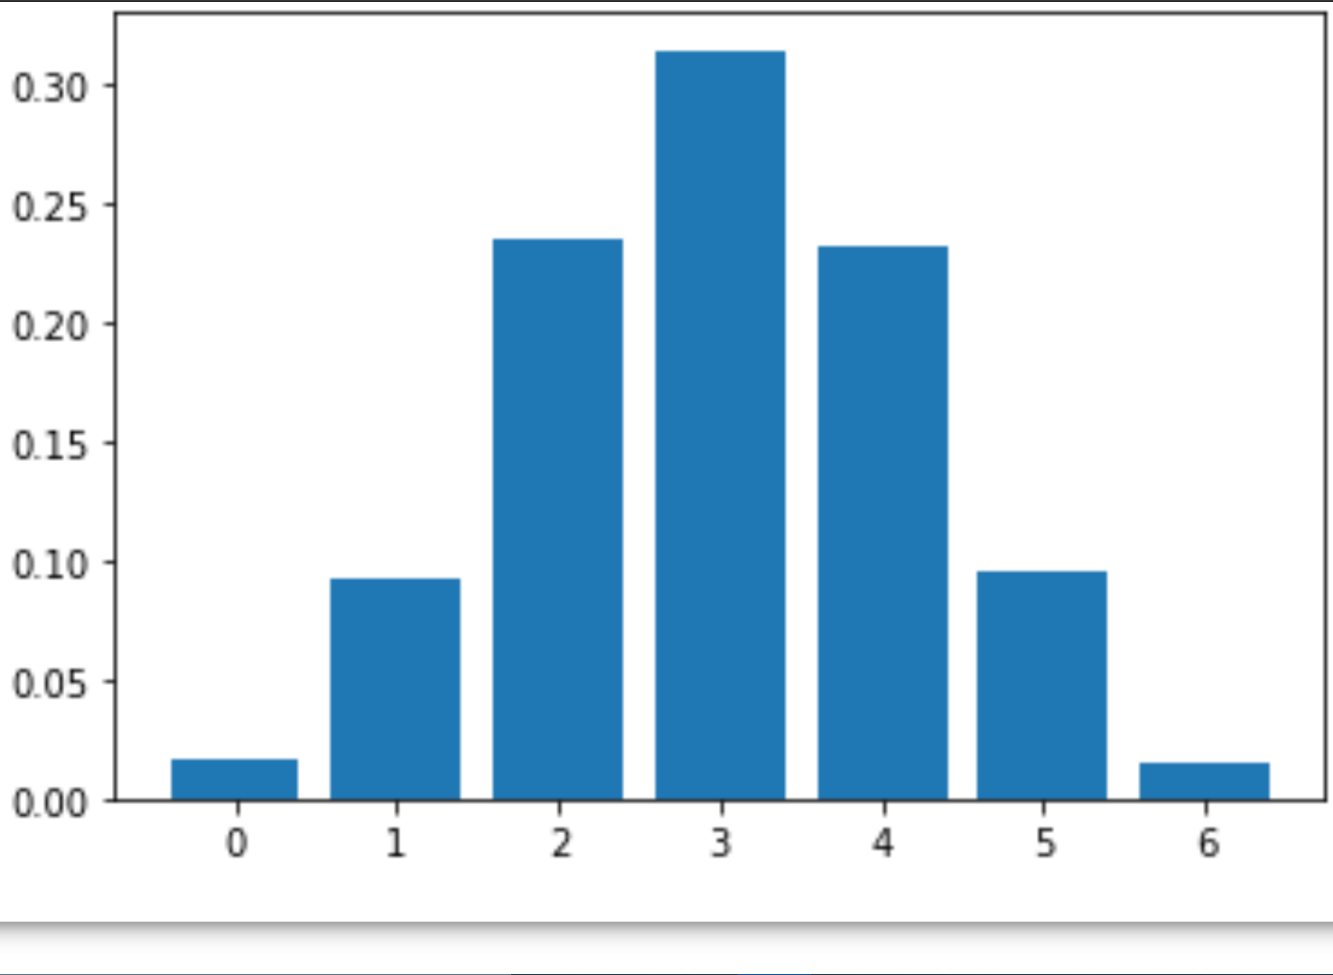
\includegraphics[scale=0.2]{images/Screenshot (184).png}
\end{center}
  

\begin{enumerate}
    \item probability of getting 5 successes
    \begin{align}
        Pr(X=r)= \binom{n}{r} p^{r}(1-p)^{n-r}
    \end{align}
    for n=6,r=5\\
    \begin{align}
        Pr(X=5)= \binom{6}{5} (\frac{1}{2})^{5}(1-\frac{1}{2})^{6-5}\\
        Pr(X=5)=\frac{3}{32}
    \end{align}
    \item probability of getting at least 5 successes
    \begin{align}
        Pr(X\geq r)=\sum ^{n}_{k=r} \binom{n}{k} p^k (1-p)^{n-k}
    \end{align}
    for n=6,r=5
    \begin{align}
        Pr(X\geq5)=\sum^6_{k=5}\binom{6}{k} (1/2)^k (1-1/2)^{6-k}\\
        =\binom{6}{5}(1/2)^5 (1/2) + \binom{6}{6}(1/2)^6 (1)\\
        =\frac{7}{64}
    \end{align}
    \item Probability of getting at most 5 successes.\\
 Using CDF\\
 \begin{align}
     F(r)=Pr(X\leq r)=\sum^{r}_{i=0}Pr(X=i)
 \end{align}
 $$
     F(r)= \begin{cases}
     \dfrac{1}{64} ,  r=0\\
     \\
     \dfrac{7}{64} , r=1\\
     \\
     \dfrac{22}{64} , r=2\\
     \\
     \dfrac{42}{64} , r=3\\
     \\
     \dfrac{57}{64} ,r=4\\
     \\
     \dfrac{63}{64} , r=5\\
     \\
     \dfrac{64}{64} , r=6\\
     \\
     
     
     \end{cases}
 $$
    \begin{align}
        F(r)= Pr(X\leq r)=\sum^{r}_{i=0}Pr(X=i)
    \end{align}\\
    for n=6,r=5
    \begin{align}
        F(5)=Pr(X\leq 5)=\sum^{5}_{i=0}Pr(X=i)\\
        =\frac{1}{64}+\frac{6}{64}+\frac{15}{64}+\frac{20}{64}+\frac{15}{64}+\frac{6}{64}\\
        =\frac{63}{64}
    \end{align}
    
    or\\
       Sum of the probabilities of all possible cases is 1\\
    \begin{align}
        \sum^{n}_{i=0}Pr(X=i)=1\\
        Pr(X\leq r)=\sum^{r}_{i=0}Pr(X=i)
    \end{align}
        from (0.0.10)\\
    \begin{align}
        \sum^{r}_{i=0}Pr(X=i)=1-\sum^{n}_{i=r+1}Pr(X=i)\\
        Pr(X\leq r)=1-\sum^{n}_{i=r+1}Pr(X=i)
    \end{align}
    for n=6,r=5
    \begin{align}
        Pr(X\leq5)=1-\sum^{6}_{i=5+1}Pr(X=i)\\
        =1-Pr(X=6)
    \end{align}
    Using (0.0.3)
    \begin{align}
       Pr(X=6)=\binom{6}{6} (1/2)^{6}(1-1/2)^{6-6}=(1/2)^6
    \end{align}
    therefore
    \begin{align}
      Pr(X\leq5)=1-(1/2)^6=\frac{63}{64}
    \end{align}
\end{enumerate}


\end{document}
